\chapter{Utilizing Onboard Compute In SteelEagle}

This chapter discusses work to replace the communications relay used in
SteelEagle to the Modal AI VOXL 2. The VOXL 2 offers significant computational
capability, allowing the execution of Tensorflow Lite machine learning models.
We start by characterizing this shift in offloading strategy in more general
terms.

\section{The Computation Offload Spectrum}
\begin{figure}[htbp]
\centerline{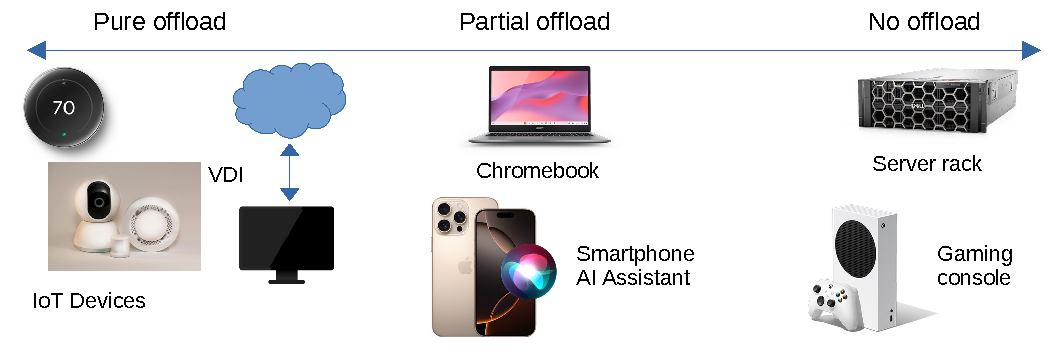
\includegraphics[width = .8\textwidth]{figs/offload-spectrum-crop.pdf}}
\caption{Devices Placed in the Computation Offloading Spectrum}
\label{fig:offload-spectrum}
\end{figure}
Devices today leverage offloading to various degrees.
\Cref{fig:offload-spectrum} shows how devices can be placed in an offloading
spectrum, with thin clients found towards the left of the spectrum and thick
clients to the right. A thin client, as opposed to a thick client, has minimal
compute and can be made smaller, lighter, and cheaper. Virtual desktop
infrastructure (VDI), for example, leverages pure offload by providing remote
access to desktops hosted on centralized servers.  This reduces the
computational demands on the client device, enabling the use of
computationally-intensive applications on weaker and older ``thin'' hardware,
reducing costs. Similarly, internet-of-things (IoT) sensors, such as video
cameras, cirumvent their limited storage and computational ability by
leveraging pure offload, transmitting their sensor streams to the cloud for
storage and analysis.

On the other end of the spectrum, we find devices such as gaming consoles,
desktop computers, and autonomous cars. Gaming consoles and desktop computers
are expected to have crisp interaction, which is not achievable by offloading
to cloud. Offloading to cloudlets, which can provide low latency, is not a
feasible option for these devices currently because of the absence of
widespread cloudlet infrastructure.  Gaming consoles and desktop computers can
provide high-levels of onboard computational power because they are not subject
to mobility constraints.  Although autonomous cars are mobile, they typically
have sufficient energy available to perform intensive onboard computations
since the majority of energy is needed to propel the car forward. They must
also perform real-time decision making reliably even in the absence of network
connectivity, which makes offloading less appealing.

In the middle of the spectrum, we find devices that perform partial offloading.
These devices have sufficient computational power to function when offloading
is unavailable or not advantageous, but they also offload computation in other
cases. Smartphone AI voice assistants such as Apple's Siri, for example,
originally offloaded all computation to the cloud. Over time, it evolved to
utilize on-device capabilities to perform simpler tasks, allowing its use in
the absence of an internet connection.  Chromebooks were designed with a focus
on the use of cloud-based services, allowing them to be fitted with lower
processing power, memory, and storage capacity compared to traditional laptops.

\subsection{How should applications decide the offloading strategy?}
\label{sec:deciding-offloading-strategy}

Choosing an offload strategy for a given application can be done based on some
key attributes that are considered important for the application:
\begin{enumerate}
    \item \textbf{Mobility requirements}: is the application subject to
        mobility constraints?
    \item \textbf{Disconnected operation}: does the application need to work reliably
        in the face of network disconnection or degradation? Is degraded operation
        acceptable during disconnected operation?
    \item \textbf{Latency requirements}: is the application latency-sensitive?
        Are there tasks that are computationally intensive but can tolerate
        high latency if a nearby cloudlet is unavailable?
    \item \textbf{Bandwidth constraints}: how much network bandwidth is
        available to the application?
    \item \textbf{Cost requirements}: is low cost for devices a priority in
        this application?
\end{enumerate}

These attributes encapsulate the benefits and limitations of offloading.
Offloading is typically only relevant for mobile devices. A mobile device that
is dependent entirely on offloading will be unable to function adequately when
offloading is impossible altogether because of network disconnection, or
impacted because of degraded network conditions, such as high latency and low
bandwidth availability. Applications that are mission-critical would be wise to
equip devices with sufficient computational resources to support an acceptable
level of function when adverse network conditions impact offloading.
Applications that are not mission-critical can rely on pure offload to benefit
from the cost savings resulting from using devices that are not required to
have significant computational resources.

Offloading allows mobile devices to achieve a much higher level of
functionality that their onboard hardware allows for. Equipping mobile devices
with the hardware needed to maintain the same level of functionality during
offload degradations reduces the benefit of offloading---the mobile device is
weighed down with the additional size and weight of more complex hardware that
remains unused when offloading is possible.

If offload degradations are infrequent, a more reasonable approach is to
utilize the inferior on-device computational resources to compute results that
are inferior according to an output-specific metric, compared to those obtained
using offloading. For predictions from a machine learning model, the metric
could be the accuracy of the prediction. In previous work, the concept of
\textit{fidelity} has been used in this context, defined as the degree to which
the results differ according to the metric \cite{noble1997}.

\subsection{The dynamic nature of partial offload}

Network conditions affect the performance of offloading, but they are dynamic
in nature. Mobile devices utilizing partial offload, then, must decide an
offloading strategy at runtime. But the decision is not binary---exclusively
using onboard compute or remote compute resources.  As
\cref{fig:offload-spectrum} shows, there is a wide range between the two ends
of the spectrum. Depending on the current network conditions, partial-offload
mobile devices can utilize a combination of onboard and remote computational
resources that results in optimal performance.

Mobile devices can achieve this through an optimal partitioning of applications
into local and remote components. Flinn et al tackled the issue of developing
applications that can support devices with different capabilities and dynamic
execution conditions with a self-tuning remote execution system. The system,
called \textit{Spectra}, continuously monitors the application's resource
supply and demand and suggests which components of an application should be
executed remotely, taking into account factors such as performance, energy
usage, and fidelity \cite{flinn2002}. This work requires the application
developer to partition the application, specifying application components
that could benefit from remote execution.

\section{A Partial Offload Pipeline for SteelEagle}

SteelEagle drones can currently be placed in the ``pure offload'' part of the
spectrum in \cref{fig:offload-spectrum}, since they do not perform any on-board
computation other than the encoding of the raw camera feed to an RTSP H.264
video stream that is transmitted to a cloudlet. As discussed in
\cref{sec:deciding-offloading-strategy}, a pure offload strategy does not
support disconnected operation, and impacts the application considerably as
network conditions degrade.

\begin{figure}[htbp]
\centerline{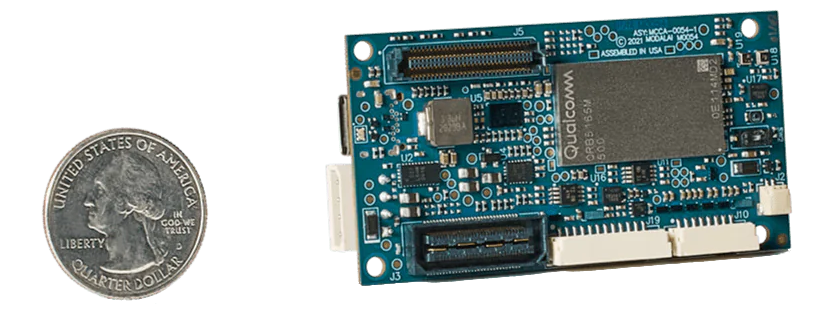
\includegraphics[width = .5\textwidth]{figs/voxl2.png}}
\caption{Modal AI VOXL 2}
\label{fig:voxl2}
\end{figure}

Replacing the Onion Omega 2 with the Modal AI VOXL 2 (\cref{fig:voxl2}) as the
communications relay in the SteelEagle pipeline will allow us to pursue a
partial offloading strategy that can allow SteelEagle drones to gracefully
react to changes in network conditions. The VOXL 2 is intended to be used as an
AI autopilot in custom drones. It features a Qualcomm QRB5165 processor, and
adds components such as a PX4 flight controller. \Cref{tab:voxl2-specs}
provides information about the computational resources available on the VOXL 2.

\begin{table}
    \centering
    \begin{tabular}{@{}ll@{}}
        \toprule
        \textbf{} & \textbf{Details}\\
        \midrule
        \textbf{CPU} & Qualcomm Kyro 585, 2.84 GHz x 8 cores\\
        \textbf{GPU} & Qualcomm Adreno 650, with support for OpenCL\\
        \textbf{DSP} & Qualcomm Hexagon 698\\
        \textbf{Weight} & 16 grams\\
        \textbf{Power consumption} & 4-5 W under high load\\
        \bottomrule
    \end{tabular}
    \caption{The specifications of the QRB5165 processor used in the VOXL 2}
    \label{tab:voxl2-specs}
\end{table}
